\chapter{Parallelization Techniques for Lattice Deformers}
\label{chp:parallelization}

In this chapter, we will explore techniques for optimizing the force
computation procedures for lattice deformers. Recall from Chapter
\ref{chp:engineering}, that our goal in solving elastic deformations
is to compute forces and force differentials from current nodal
positions. We codified this process in Algorithm
\ref{alg:isotropicforces}, where we detailed the computational steps
required for converting nodal positions into the corresponding nodal
forces according to a material specific energy function. The important
take away from this algorithm is that we are able to compute these
forces on a per cell basis. On the surface, this would seem to be an
excellent opportunity for thread-based parallelism: divide all the
cells among available processor cores and have each core operate on
its cells in isolation. Unfortunately, this is where we run into
problems.

The first problem is that while all cells are functionally
independent, the nodes themselves are not. When we compute forces on
nodes, we are actually producing aggregate forces. That is, for any
node in the lattice, we are interested in sum of all forces from all
cells it is connected with. By using thread-based parallelism, we
encounter a significant problem.  In the context of a single thread,
the processing of cells is serial. But when two or more threads, each
operating on different cells, try to accumulate to a single node we
encounter a serious \textit{write hazard}. In this case, the hazard is
that we don't have any guarantees that our final result will be the
sum of all forces from all involved cells. Due to the behaviors of the
processor caches and system memory, we might have a result equal to
any one single cell's result, any combination of the cells combined,
or some unrelated value. We could attempt to remove this confusion by
adding a locking protocol around each node, but this would introduce
significant performance penalties.

The second problem we encounter is when reading and writing nodal
information. In Chapter \ref{chp:nonmanifold}, we demonstrated how
non-manifold embedding meshes could be constructed to represent
material geometry with thin features or incisions. However, this
approach comes with a significant drawback: The explicit topology
required to define the mesh removes much of the regularity we could
otherwise depend on for performance. One nice benefit of using an
implicit topology for our lattices is that the memory locations of all
cells and nodes can be quickly computed via a function of their
geometric positions. This allows reading and writing to these
locations to be done via a single memory access: the exact storage
location. In contrast, the explicit topology we constructed
previously has no such guaranteed relationship between storage
locations and geometric positions. Instead it uses an explicit record
of pointers for each cell that informs us where the memory is
stored. This can hurt performance in two ways: first, there is no
guarantee that memory is well ordered. Neighboring geometric nodes
might be arbitrarily far apart in memory. Since modern processors load memory in
linear strips, known as cache lines, this distance might require
multiple loads, where a single load might have sufficed if they were
closer. Second, by using a collection of pointers per cell, we are
actually reading twice for every entry. The first read is to load the
value of the pointer, followed by the data itself. Combined, these
memory access issues can be extremely detrimental to performance,
especially since modern processors operate in a regime of roughly two
orders of magnitude more available computational resources than memory
access rate. Despite the significant number of numerical steps
required to process each cell, any delays in memory access could lead
to the computation becoming memory bound.

We can deal with these problems by more carefully arranging our data
for computation. Our proposed solution makes use of two concepts:
hybrid grids and blocking. Along the way, we will also show how C++
templates can be employed for guiding SIMD vectorization of
blocks. The following sections will cover these concepts in more detail.

\section{A hybrid embedding lattice structure}
\label{sec:hybrid}

We build on the non-manifold embedding mesh concepts discussed in
Chapter \ref{chp:nonmanifold}, but now we seek to optimize these
data structures for computational performance. Although the use of
non-manifold embedding meshes recovers much of the topological
expressive ability of conforming meshes, it jeopardizes one of the
most attractive features of regular embedding lattices, the fact that
connectivity is implicit in the lattice structure as opposed to
explicitly stored in a mesh. The performance impact of implicitly
defined topology can be profound; the memory footprint of explicitly
stored connectivity information can easily exceed the state variables
themselves (e.g. nodal positions) and reduce effective memory
bandwidth by necessitating indirect memory access. In this section, we
strive to leverage the best of both worlds: We use an (implicit
topology) Cartesian grid to capture the majority of the embedded model
in regions where non-manifold duplication is not needed. We retain the
topological flexibility of non-manifold embedding lattices by
hybridizing this grid with an (explicit topology) hexahedral mesh used
to describe regions in the vicinity of narrow slits and incisions.


% \begin{figure}
% \centering
% \subfloat{
% \includegraphics[height=.2\paperheight]{chapter_gridiron/example_images/Single_zPlasty_1/embedded/render0057.png}
% \hfill
% \includegraphics[height=.2\paperheight]{chapter_gridiron/example_images/Rhomboid_Scalp_1/embedded/render0010.png}
% }

% \subfloat{
% \includegraphics[height=.2\paperheight]{chapter_gridiron/example_images/Single_zPlasty_1/embedded/render0071.png}
% \hfill
% \includegraphics[height=.2\paperheight]{chapter_gridiron/example_images/Rhomboid_Scalp_1/embedded/render0022.png}
% }

% \subfloat{
% \includegraphics[height=.2\paperheight]{chapter_gridiron/example_images/Single_zPlasty_1/embedded/render0093.png}
% \hfill
% \includegraphics[height=.2\paperheight]{chapter_gridiron/example_images/Rhomboid_Scalp_1/embedded/render0046.png}
% }

% \subfloat{
% \includegraphics[height=.2\paperheight]{chapter_gridiron/example_images/Single_zPlasty_1/lattice/render0071.png}
% \hfill
% \includegraphics[height=.2\paperheight]{chapter_gridiron/example_images/Rhomboid_Scalp_1/lattice/render0022.png}
% }

% \vspace*{-.08in}
% \caption{Simulation of Z-Plasty and Rhomboid flap repairs}{Left:
%   Simulation of \textbf{Z-Plasty}, a basic maneuver resulting in
%   anisotropic scaling along two perpendicular directions. Z-Plasty is
%   a common building block leveraged in more elaborate repairs. Right:
%   \textbf{Rhomboid flap} procedure for closing a quadrilateral
%   aperture of excised tissue on the scalp. The embedded simulation
%   grids are shown on the right.}
% \label{fig:Zplasty-RhomboidScalp}
% \vspace*{-.16in}
% \end{figure}


% \begin{figure}
% \centering
% \subfloat{
%  \includegraphics[width=.35\paperwidth]{chapter_gridiron/example_images/Dual_sPlasty_Scalp_1/embedded/render0023.png}
% \hfill
% \includegraphics[width=.35\paperwidth]{chapter_gridiron/example_images/Dual_sPlasty_Scalp_1/embedded/render0066.png}
% }

% \subfloat{
% \includegraphics[width=.35\paperwidth]{chapter_gridiron/example_images/Dual_sPlasty_Scalp_1/embedded/render0115.png}
% \hfill
% \includegraphics[width=.35\paperwidth]{chapter_gridiron/example_images/Dual_sPlasty_Scalp_1/lattice/render0066.png}
% }
% \vspace*{-.1in}
% \caption{Simulation of a Dual S-Plasty repair on the scalp}{\textbf{Dual S-Plasty} procedure on the scalp; a large oval-shape defect is patched by transposing two S-shaped flaps.}
% \label{fig:SPlasty-Scalp}
% \vspace*{-.15in}
% \end{figure}

\subsection{Reduction and Remapping}

To transform an explicit non-manifold mesh into a hybrid grid, we
attempt to map as much of the explicit-connectivity mesh as possible
back onto an implicit-connectivity grid to recover regularity. From
the explicit mesh, we have two geometric primitives to consider for
remapping: nodes and cells. For simplicity, we will first consider
nodes and then cells. Figure \ref{fig:remapping} illustrates the
results of the remapping rules below:
\begin{itemize}
\vspace*{-.05in}\item Nodes are mapped to the grid if and only if they possess no duplicates.
\vspace*{-.05in}\item Cells are mapped to the grid if and only if all of their vertices have been mapped to the grid.
\end{itemize}
\vspace*{-.05in} Each mesh cell remaining in the hybrid lattice is
associated with a coordinate from the grid. This mapping will become
important later when we discuss the block-based acceleration
structures.  After these rules are applied, the new structure must
adhere to several post-conditions.
\begin{itemize}
\vspace*{-.05in}\item All grid cells are composed only of grid nodes.
\vspace*{-.05in}\item Mesh cells contain one or more mesh nodes.
\end{itemize}
It should be noted that this set of rules is not strictly optimal in
the sense of mapping the most elements into the grid. A more
aggressive strategy would be to select one element from each set of
geometrically co-located items and map it to the grid. We defer
investigation of similar compaction heuristics to future work.
\textbf{Note:} In these surgical examples (Figure \ref{fig:surgicalembeddings}) mesh-mapped embedding cells are indicated
with blue color, grid-mapped ones in red. Typically, only a minority
of cells is mesh-mapped, allowing us to retain the bulk of performance
benefits of implicit grid-mapped embeddings.


\begin{figure}
  \centering
\vspace*{-.12in}
  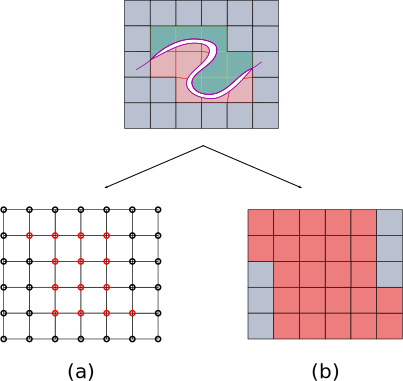
\includegraphics[width=3in]{chapter_gridiron/images/Figure_Topology_D}
\vspace*{-.07in}
  \caption{Illustration of cell type categorization}{From an explicit mesh (top), we generate (a) mesh mapped nodes in red, grid mapped nodes in black and (b) mesh mapped cells in red, grid mapped cells in gray.}
  \label{fig:remapping}
\end{figure}

\begin{figure}
  \centering
  \includegraphics[width=.32\paperwidth]{chapter_gridiron/example_images/Dual_sPlasty_Scalp_1/lattice/render0066.png}
  \includegraphics[width=.32\paperwidth]{chapter_gridiron/example_images/Single_zPlasty_1/lattice/render0071.png}
  \includegraphics[width=.32\paperwidth]{chapter_gridiron/example_images/Rhomboid_Scalp_1/lattice/render0022.png}
  \caption{Embedding discretizations of surgical operations}{Three
    different surgical operations, S-Plasty (Top Left), Z-Plasty (Top
    Right), and a Rhomboid Flap (Bottom), are shown with their
    embedding hybrid grids. Cells in red are part of the grid region, while
    blue cells are mesh mapped. Green cells mark Dirichlet regions.}
  \label{fig:surgicalembeddings}
\end{figure}

\section{Parallelization}

\begin{algorithm}
  \caption{General Parallelization Design Strategy}
  \label{alg:GeneralStrategy}
  \begin{algorithmic}[1]

    \For{ $t = 0 \ldots N$ }

    \State $\{ o_1(t), o_2(t),\ldots, o_m(t) \} = \Call{Kernel}{\{ i_1(t), i_2(t),\ldots, i_n(t) \}}$
    
    \EndFor
    
  \end{algorithmic}
  
\end{algorithm}


Our framework relies on both multithreading and vectorization (SIMD)
to obtain the best possible performance. The fact that our
Cartesian-based discretization consists of identically shaped elements
offers a great opportunity to leverage both thread-level and
data-level parallelism, due to the inherent regularity of the
simulation kernels. Our general strategy is to design operations that
resemble the form shown in Algorithm \ref{alg:GeneralStrategy}. Under
this approach, our numerical kernels for computing nodal values
operate on multiple streams of input data,
$\{ i_1, i_2,\ldots, i_n \}$, and produce multiple streams of output
data, $\{ o_1, o_2,\ldots, o_m \}$. Collections of streams can be
grouped together logically into vectors or matricies. By structuring
the computation in this form, we can clearly see where multithreading
and vectorization apply: Each thread will be assigned a partition over
$N$, while vectorization can be used to execute multiple instances of
\textsc{Kernel} by stepping through the partition in strides. This
also suggests a data structure design: Arrays of Structs of Arrays
(AoSoA), where each struct contains the data for each computational
stride and the array of structs can be divided evenly between
threads. In the next couple of sections, we will look at how the
simulation data, currently arranged in a hybrid grid, can be
repackaged according to the AoSoA methodology, a process called blocking. 

\begin{algorithm}
\caption{SIMD Compatible Block Construction}
\label{alg:BlockGeneration}
\begin{algorithmic}[1]
\Require Block region $i$
\Function{GenerateBlocks}{}
  \ForAll { Cell $c$ in $i$ }
    \State Create new empty block
    \State Copy $c$ into new block
  \EndFor
  \State Build connectivity graph between blocks
  \Repeat
    \ForAll{Symmetric connected block pairs}
      \State Find pair with fewest neighbor mismatches
    \EndFor
    \If{Suitable pair found}
      \State Collapse, merging block contents
     \EndIf
  \Until{No further collapses occurred}
  \State \Return All remaining blocks
\EndFunction
\Ensure A collection of one or more manifold Blocks
\end{algorithmic}
\end{algorithm}


\subsection{Blocking}

As described in Section \ref{sec:engineering:discreteformulas} and Algorithm
\ref{alg:isotropicforces}, forces are computed on a per cell basis. A naive
multithreaded port would result in write hazards at nodal positions,
unless expensive synchronization was used. Simple partitioning would
eliminate this issue, but would not make efficient use of
modern SIMD-enabled processors. Instead, we employ a blocking scheme to avoid write
hazards while retaining a memory layout favorable for
vectorization. Our objective is to redefine our ``quantum'' of
computation from a single lattice cell, to a geometric neighborhood
(or \emph{block}) that is processed concurrently using vector
  operations.  We adopt a block size of eight cells
arranged as a $2\times 2\times 2$ cube. This formation
allows us to fit blocks into eight\char`-wide
vectors and later we will demonstrate how we can
adapt to larger and smaller vector widths. In this way,
each cell in the block can be considered a ``channel'' in the
vector.  Blocks are tiled together to cover the
  extent of the lattice. However, restricting the contents of a
  non-manifold hybrid lattice to the spatial extent of a single block
  could easily yield more than one cell at each position in the block,
  as illustrated in Figure \ref{fig:blocking}. To create blocks
  without overlapping cells, we employ a greedy algorithm which
  collects cells into manifold groupings along block boundaries, as
  seen in (Figure \ref{fig:blocking}c). The full algorithm for this
  process is described in Algorithm \ref{alg:BlockGeneration}.


\label{sec:blocking}
\begin{figure}[b!]
  \centering
  \def\svgwidth{\columnwidth}
  \vspace*{-.15in}
  \input{chapter_gridiron/images/New_Blocking.pdf_tex}
\vspace*{-.5in}
\caption{Illustration of blocks formed from regions of manifold connectivity}{Generating Blocks. (a) Block boundaries superimposed over
hybrid lattice. (b) Non-manifold contents of each block region. (c)
Final manifold blocks for each region.}
\label{fig:blocking}
\end{figure}
  
\begin{figure}[t]
   \includegraphics[width=\textwidth]{chapter_elasticity/figures/simd.pdf}
   \vspace*{-.3in}
   \caption{Illustration of data structure optimized for vector
     hardware}{A 2D illustration of our simulation data
     structures. Left: Nodal (deformation) data stored on a
     grid. Middle: On demand, nodal data is copied to an array of
     $2^d$-sized blocks and combined with cell-based data which are
     persistently stored in arrays of blocks. Right: Nodal and
     cell-centered data for a single block are copied to a
     stack-allocated structure, and duplicated for each voxel for SIMD
     computation.}
   \label{fig:simd}
   \vspace*{-.15in}
\end{figure}
  
We use the partitioning of our lattice into blocks to circumvent write
dependencies during multithreaded execution. Our approach is
illustrated in figure \ref{fig:simd}. Prior to the execution of any
kernel involving force computation, we copy the state variables from
either the grid or mesh structures that natively store them, into
duplicate copies for every block. We label this process a
\textbf{Compaction} step, which is essentially a \emph{gather}
operation that yields a representation of the state variables into a
flattened array of blocks (with shared variables duplicated across
blocks). Of course, this step entails creating multiple copies of
data, but is not as expensive as if a separate copy of all nodal data
was made for every individual voxel (the practical data overhead is
$<3x$ for this scheme, compared to $8x$ for a replication of all nodes
for all cells). The cost of this data duplication is reduced by the
fact that additional simulation meta-data (material parameters,
precomputed stress derivatives and Singular Value/Polar
decompositions, if needed) which are conceptually cell-centered can be
stored \emph{persistently} in a flattened array of blocks. Once this
translation is completed, fully balanced multi-threading is possible
by simply subdividing the processing of this flattened array across
computing threads. Within each thread, we leverage the $2^3$
multiplicity of each block to compute differentials with SIMD
instructions. The blocks of nodal and cell data are first copied from
the heap-allocated flat arrays onto a stack-allocated copy. Then, we
perform a final separation of cell and node data, creating one fully
separate copy for each of the 8 voxels. Note that this operation does
not incur memory bandwidth expense, since this local stack-allocated
copy (typically less than $6-8KB$ in size) is expected to be
cache-resident for the duration of the computation. We have leveraged
the AVX instruction set available in modern Intel CPU architectures to
process all 8 voxels of the block simultaneously. Subsequently, force
computation can be executed in parallel on each block, without write
dependencies, by allowing each block to record its own force
contribution to the lattice nodes it touches. Upon completion of the
local computation, the reverse operation, labeled
\textbf{Uncompaction}, scatters and accumulates the contents of the
per-block forces back to their native (non-duplicated) grid or mesh
storage. Write dependencies can be avoided at this stage by
partitioning this parallel operation on the grid or mesh variables
that collect the per-block contributions. As a result, complex force
computations can fully enjoy the benefits of thread- and
SIMD-parallelism, without being concerned with data dependencies
arising from the non-manifold mesh structure.

\subsection{Supporting Irregular Cells}

In simple cases, where all cells are composed of material or not, the
previous approach for data organization works well. Even for cases
where cells are allowed to be practically full of material, we can
simply adjust the force computation \citep{PatteMS:2012}. While this
increases the complexity, it does so in a uniform fashion - all cells
become more complex. The true enemy of vectorization is
irregularity. Unfortunately, when we are faced with features like
point spring constraints and optional material layering, useful in
adding non-uniform, local anisotropic behaviors like muscle fiber
effects, we quickly encounter cells which require more or less
computation than their neighbors. Fortunately, we can adapt the
blocking approach to handle this situation with a few minor
modifications.

The primary idea we will use in this situation is the concept of a
\textit{block overlay}. A block overlay is additional metadata applied
to each block to handle optional force generating components. For each
block which contains any irregular cells, we can build a block overlay
data structure which contains additional per cell data. The exact
description of each overlay varies, depending on its reason for
existence. For instance, a spring constraint overlay would contain
embedding weights and a spring stiffness coefficient for each cell
with an embedded spring. By building these overlay structures at the
level of whole blocks, we can easily integrate them with the
thread-parallelized loop over all blocks. In order to handle cells
with more than one special feature ( e.g. it is reasonable to have
more than one spring constraint per cell), we can repeat the same idea
we used earlier when constructing the block layouts. In this case, we
attempt to pack block overlays as full as possible, as long as each
cell in the overlay has at most one special feature. Thus, we will
generate as many block overlays as the most complex cell in the block,
where the worst case is that only one cell in the overlay has non-null
data. The drawback of this approach is that we have now have some
amount of variable processing per block, given an arbitrary number of
overlays, but computing each overlay's contribution can be done in a
vectorized fashion. The entire breakdown of the process, over multiple
blocks with overlays, can be seen in Figure \ref{fig:full-block-vectorization}.

\begin{figure}[t]
   \includegraphics[width=\textwidth]{chapter_elasticity/figures/full-block-vectorization.png}
   \vspace*{-.3in}
   \caption{Illustration of data structure optimized for vector
     hardware, with overlays}{A complete 2D illustration of the block
     based vectorization computation of elastic forces, including
     irregular cell data overlays. From top to bottom: Gathering
     positional data from hybrid grid cells, combining with cell
     centered metadata for elastic force computation, adding block
     dependent overlays for force constraints and local material
     mix-ins, final forces are scattered back to hybrid mesh.}
   \label{fig:full-block-vectorization}
   \vspace*{-.15in}
\end{figure}


\subsection{Guided Vectorization}

The high degree of regularity exposed by our blocking procedure
naturally suggests using modern processor's SIMD capabilities to
compute on all cells of a given block simultaneously. Although the
performance potential is undeniable, porting code from a scalar
implementation to a SIMD platform is a tedious task, one that
auto-vectorization features of compilers have been traditionally
ineffective in providing automatically (especially for
large kernels, as the ones in our solver, which might contain
thousands of machine instructions for processing forces on a
single cell). An example is the highly optimized SVD routines,
published with the work of \citet{McAdaZSETTS:2011} which replicates almost
instruction-by-instruction identical SIMD intrinsics to implement
scalar, SSE and AVX versions; it can be easily verified that
compiler auto-vectorization cannot provide competitive performance
with these tediously hand-optimized kernels.

We have designed a programming paradigm called \emph{guided
  vectorization}, with which we practically achieve the performance of
hand-vectorized kernels, while only providing a single specification
for scalar \emph{and} vector variants. Our solution is object-oriented
and based on the observation that the semantics of fundamental data
types are very similar across scalar/vector platforms, even if the
interface differs. Our system is rooted on two templatized C++
classes:
\begin{shaded}
\texttt{template<class scalar\char`_arch> class Number;}
\end{shaded}

\begin{shaded}
\texttt{template<class boolean\char`_arch> class Mask;}
\end{shaded}
\vspace*{-.1in} Class \texttt{Number} is an abstraction of a single
floating point number in a scalar platform
(\texttt{scalar\char`_arch==float}) or of a 4/8/16-wide vector
register in SSE/AVX/Xeon Phi platforms
(\texttt{scalar\char`_arch:=\char`_\char`_mm128|\char`_\char`_mm256|\char`_\char`_mm512}). Similarly,
class \texttt{Mask} is an abstraction of the result of a comparison
operation, in a form that can be used to perform a conditional
assignment; thus \texttt{Mask<bool>} encapsulates a single C++ boolean
variable, \texttt{Mask<\char`_\char`_mm256>} captures a 256-bit mask
usable in AVX \texttt{BLEND} instructions, while
\texttt{Mask<\char`_\char`_mmask16>} encapsulates the special concept
in Intel Xeon Phi of a 16-bit \emph{mask register} that is used in
comparisons and conditional assignments. We provide enough overloaded
operators in the interface of these classes to allow them to be used
in algebraic expressions regardless of the encapsulating vector
width. Ultimately we use them to construct macroscopic kernels of the
form:
\begin{shaded}
\texttt{template<class \changed{scalar\char`_arch}{ Tw},class T\char`_DATA\oldtext{=void}>}\\
\texttt{void Add\char`_Force\char`_Differential(}\\
\texttt{\hspace*{2em}const T\char`_DATA (\&dx)[3][8], ...}\\
\texttt{\hspace*{2em}const T\char`_DATA (\&V)[9],}\\
\texttt{\hspace*{2em}const T\char`_DATA (\&dPdF)[12],}\\
\texttt{\hspace*{2em}T\char`_DATA (\&df)[3][8]);}
\end{shaded}
These kernels are broken out in Figures \ref{fig:KernelUPBS},
\ref{fig:KernelAF}, and \ref{fig:KernelAFD}.

In this paradigm, we have separated the programmatic
data width (\oldtext{encapsulated by }type
\texttt{T\char`_DATA}\newtext{, which could be \texttt{float}, for
  scalar code that computes forces on individual cells, or
  \texttt{float[8]}, for the force computation of all 8 cells of a
  block at once}) from the architectural vector width. This allows us
to\changed{ design all of}{ program all} these kernels with the same
semantics that would be followed for scalar execution, and
automatically generate code that works on geometric blocks of any
size, and vector architectures of different vector widths. For example
the function call
\texttt{Add\char`_Force\char`_Differential<\char`_\char`_m128,float[16]>(....)}
would use SSE instructions to compute force differentials of geometric
blocks containing 16 cells each (e.g. blocks shaped like
$4\times 2\times 2$ grid cells). 


\subsection{Performance Results}

This particular strategy for performance optimization for lattice
deformers was tested in a prototype surgical simulation tool (For more
details, see Chapter \ref{chp:deployment} on its deployment). In
addition to the surgical models simulated with this tool, we also
benchmarked our system with a high resolution human body model with
anisotropic active musculature. Detailed timings, including
time taken at the individual kernels of our solver, can be seen in Table
\ref{fig:TimeResultsTable}.


% \begin{figure}[t]
% \centering
% \caption{\textbf{Classification of Forces:} The energy, $\mathbf{E}$, of deformable objects in our framework can be expressed as a summation of independent components. Additionally, we classify these components' related forces into general categories.}

% $$
% \mathbf{E} = \mathbf{E}_{iso} + \mathbf{E}_{aniso} + \mathbf{E}_{stab} + \mathbf{E}_{con} + \mathbf{E}_{coll}
% $$

% \scalebox{1.5}{$\Downarrow$}

% \begin{forest}
% [All Forces
% [Elasticity
% [Isotropic]
% [Anisotropic]
% [Stabilization]
% ]
% [Interactions
% [Constraints
% [Unilateral]{\draw[->,dashed] ()--++(0pt,-.5cm)--++(3.33cm,0pt) to (rb);}
% [Bilateral]{\draw[->,dashed] () --++(0pt,-.75cm)--++(3.14cm,0pt) to (self);}
% ]
% [Collisions
% [Rigid Body,name=rb]
% [{\color{gray}Self},rectangle,draw,gray,name=self,edge={dashed,gray}]
% ]
% ]
% ]
% \end{forest}
% \label{fig:classification}
% \end{figure}

\begin{rotatedfigure}
  \centering
  \caption{Kernel Components for \textsc{Update Position Based State}}{Diagram
    demonstrating the sub-kernel components for the \textsc{Update Position
    Based State} kernel. This kernel is executed once per Newton step
    and computes the deformation gradient $\bm F$, the Singular Value
    Decomposition  of $\bm F$, and the stress tensor $\mathcal
    T$, as of \citet{TeranSIF:2005}, of the current configuration. These
    values can be reused in subsequent force differential computations as
    they do not change between Newton steps.}
  \vspace {.5cm}
  
  \begin{forest}
    for tree={
      child anchor=west,
      parent anchor=east,
      grow'=east,
      text width=4cm,%
      draw,
      anchor=west,
      edge path={
        \noexpand\path[\forestoption{edge}]
        (.child anchor) -| +(-5pt,0) -- +(-5pt,0) |-
        (!u.parent anchor)\forestoption{edge label};
      },
    }
    [Update Position Based State
    [Unweighted Gradient]
    [Singular Value Decomposition]
    [Penalty Measure Gradient]
    [Isotropic Stress Derivative
    [Rotated Stress Derivative]
    ]
    ]
  \end{forest}
  \label{fig:KernelUPBS}
\end{rotatedfigure}

\begin{rotatedfigure}
  \centering
  \caption{Kernel Components for \textsc{Add Force}}{Diagram demonstrating the
    sub-kernel components for the \textsc{Add Force} kernel. This kernel
    produces nodal forces due to a single cell's nodal deformation. It
  is called once per Newton step as the right hand side of the update
  expression \ref{equ:newtonupdate}.}

\vspace{.5cm}
  
  \begin{forest}
    for tree={
      child anchor=west,
      parent anchor=east,
      grow'=east,
      text width=4cm,%
      draw,
      anchor=west,
      edge path={
        \noexpand\path[\forestoption{edge}]
        (.child anchor) -| +(-5pt,0) -- +(-5pt,0) |-
        (!u.parent anchor)\forestoption{edge label};
      },
    }
    [Add Force
    [Unweighted Gradient]
    [Matrix Times Transpose]
    [Piola Kirchhoff Stress Tensor
    [Volume Preservation Deviation]
    ]
    [Unweighted Accumulation]
    ]
  \end{forest}
  \label{fig:KernelAF}
\end{rotatedfigure}

\begin{rotatedfigure}
  \centering

  \caption{Kernel Components for \textsc{Add Force Differential}}{Diagram
    demonstrating the sub-kernel components for the \textsc{Add Force
    Differential} kernel. This kernel is called repeatedly during each
    Newton step, acting as the effect of multiplying by the stiffness
    matrix $\bm K$. This kernel consumes the deformation gradient, SVD
    components, and the stress tensor $\mathcal T$ produced from the Update
    Position Based State kernel.}

  \vspace{.5cm}
  
  \begin{forest}
    for tree={
      child anchor=west,
      parent anchor=east,
      grow'=east,
      text width=4cm,%
      draw,
      anchor=west,
      edge path={
        \noexpand\path[\forestoption{edge}]
        (.child anchor) -| +(-5pt,0) -- +(-5pt,0) |-
        (!u.parent anchor)\forestoption{edge label};
      },
    }
    [Add Force Differential
    [Unweighted Gradient]
    [Matrix Times Transpose]
    [Pressure Force Differential]
    [Stress Tensor Differential]
    [Matrix Transpose Times]
    [Unweighted Accumulation]
    ]
  \end{forest}
  \label{fig:KernelAFD}
\end{rotatedfigure}

\renewcommand{\arraystretch}{1.0}

\begin{myrotatedtable}
\centering
\setlength\fboxsep{0pt}
\setlength\fboxrule{0.25pt}
\begin{tabular}{ >{\arraybackslash}m{2.5cm} >{\centering\arraybackslash}m{1cm} 
m{1.5cm} 
m{1.5cm} 
m{1.5cm} 
m{1.7cm} 
m{1.6cm} 
m{1.5cm} 
m{1.5cm} 
m{1.3cm}
 >{\centering\arraybackslash}m{1.8cm} >{\centering\arraybackslash}m{2cm}}
\toprule
\textbf{\small{Example}}  & \textbf{\small{Plat.}}        & \textbf{\small{Total Voxels}} & \textbf{\small{Grid Voxels}}   & \textbf{\small{Mesh Voxels}}  & \textbf{\small{Blocks}}   & \textbf{\small{Newton}}\newline \textbf{\small{Iteration}} \small{(s)}                       & \textbf{\small{Update}}\newline \textbf{\small{State}} \small{(ms)}                          & \textbf{\small{Add}}\newline \textbf{\small{Force}} \small{(ms)}                         & \textbf{\small{Add}}\newline \textbf{\small{Differ.}} \small{(ms)}                  & \textbf{\small{Compact}} \small{(ms)}     & \textbf{\small{UnCompact}} \small{(ms)}                                \\
\midrule
\multirow{4}{*}{\parbox{1.5cm}{\small{Dufourmentel Mouly}}}                                  & \multirow{2}{*}{Xeon} & 47689                 & 47206   & 483    & 8821   & 0.3630  & 1.5   & 1.4   & 1.6   & 0.4  & 0.6  \\
                                                                                     &                       & 294248                & 294015  & 233    & 47681  & 2.0648  & 7.8   & 5.1   & 4.2   & 2.1  & 3.0  \\
\cmidrule{2-12}
                                                                                     & \multirow{2}{*}{Phi}  & 47689                 & 47206   & 483    & 8821   & 0.4259  & 1.3   & 1.5   & 0.9   & 0.1  & 2.0  \\
                                                                                     &                       & 294248                & 294015  & 233    & 47681  & 0.7349  & 2.8   & 3.3   & 2.2   & 0.7  & 4.7  \\
\midrule
\multirow{4}{*}{\parbox{1.5cm}{Rhomboid Flap}}                                       & \multirow{2}{*}{Xeon} & 48529                 & 47203   & 1326   & 6909   & 0.1620  & 1.1   & 0.9   & 0.7   & 0.2  & 0.4  \\
                                                                                     &                       & 879571                & 877362  & 2209   & 112302 & 2.4131  & 18.4  & 9.6   & 9.0   & 3.2  & 4.0  \\
\cmidrule{2-12}
                                                                                     & \multirow{2}{*}{Phi}  & 48529                 & 47203   & 1326   & 6909   & 0.3735  & 1.3   & 1.4   & 1.0   & 0.1  & 1.5  \\
                                                                                     &                       & 879571                & 877362  & 2209   & 112302 & 1.1323  & 5.3   & 6.2   & 3.9   & 1.2  & 9.6  \\
\midrule
\multirow{4}{*}{\parbox{1.5cm}{ZPlasty}}                                             & \multirow{2}{*}{Xeon} & 54003                 & 49306   & 3697   & 6943   & 0.2293  & 1.2   & 0.5   & 0.9   & 0.3  & 0.5  \\
                                                                                     &                       & 960810                & 957908  & 2902   & 127070 & 2.7707  & 20.5  & 9.3   & 10.1  & 3.6  & 4.5  \\
\cmidrule{2-12}
                                                                                     & \multirow{2}{*}{Phi}  & 54003                 & 49306   & 3697   & 6943   & 0.3814  & 1.3   & 1.4   & 1.1   & 0.1  & 1.5  \\
                                                                                     &                       & 960810                & 957908  & 2902   & 127070 & 1.2401  & 5.9   & 6.8   & 4.3   & 1.3  & 10.8 \\
\midrule
\multirow{2}{*}{\parbox{1.5cm}{Human}}                                               & Xeon                  & 2006903               & 2006903 & 0      & 265078 & 12.112  & 35.9  & 21.5  & 20.8  & 8.4  & 12.0 \\
\cmidrule{2-12}
                                                                                     & Phi                   & 2006903               & 2006903 & 0      & 265078 & 3.9608  & 11.4  & 16.3  & 7.8   & 3.3  & 16.2 \\
\bottomrule
\end{tabular}
\vspace*{-.05in}
\caption{Performance results for surgical and animation examples.}{Examples run on the Xeon platform used a 6-core Intel Xeon CPU E5-1650 machine with 64 GB of memory, while the Phi examples ran
  on a 60-core Xeon Phi 5110P card with 8GB of memory.
% All numbers shown were run with maximum number of available cores.
%The \textsf{Update State} step consists of operations including computing  stress derivatives and taking an SVD of the deformation gradient. The \textsf{Add Force} and \textsf{Add Differentials} are responsible for computing forces and force differentials, respectively.
All surgical examples were run with 50 conjugate gradient iterations while the human example was run with 100 iterations.
%Each CG iteration consisted of a single \textsf{Add Differential} plus a \textsf{Compact} and \textsf{UnCompact}, which are described in Section \ref{sec:blocking}
} 
\label{fig:TimeResultsTable}
\vspace{-.15in}
\end{myrotatedtable}

\renewcommand{\arraystretch}{1}


%%% Local Variables:
%%% mode: latex
%%% TeX-master: "../document"
%%% End:
